\part{Session 1}
\lstset{language=C++}

\section{Introduction}
\subsection{What is mbed}
\begin{frame}
	\frametitle{What is mbed}
	The mbed development platform is a collection of open source hardware and software to allow rapid ARM based prototyping.
	\begin{itemize}
		\item Professional online compiler lets you work from any computer
		\item Integrated version control system lets you easily find and use open source libraries
		\item CMSIS based APIs for core and peripheral functions let you work high level or bare metal
		\item Hardware abstraction layer insulates your application code from hardware changes
	\end{itemize}
	\textit{Essentially a high performance Arduino with highly integrated tools to save you time}
\end{frame}

\begin{frame}
	\frametitle{Register on mbed}
	\begin{columns}[c]
		\begin{column}{0.5\textwidth}
			%TODO Edit mbed_register
			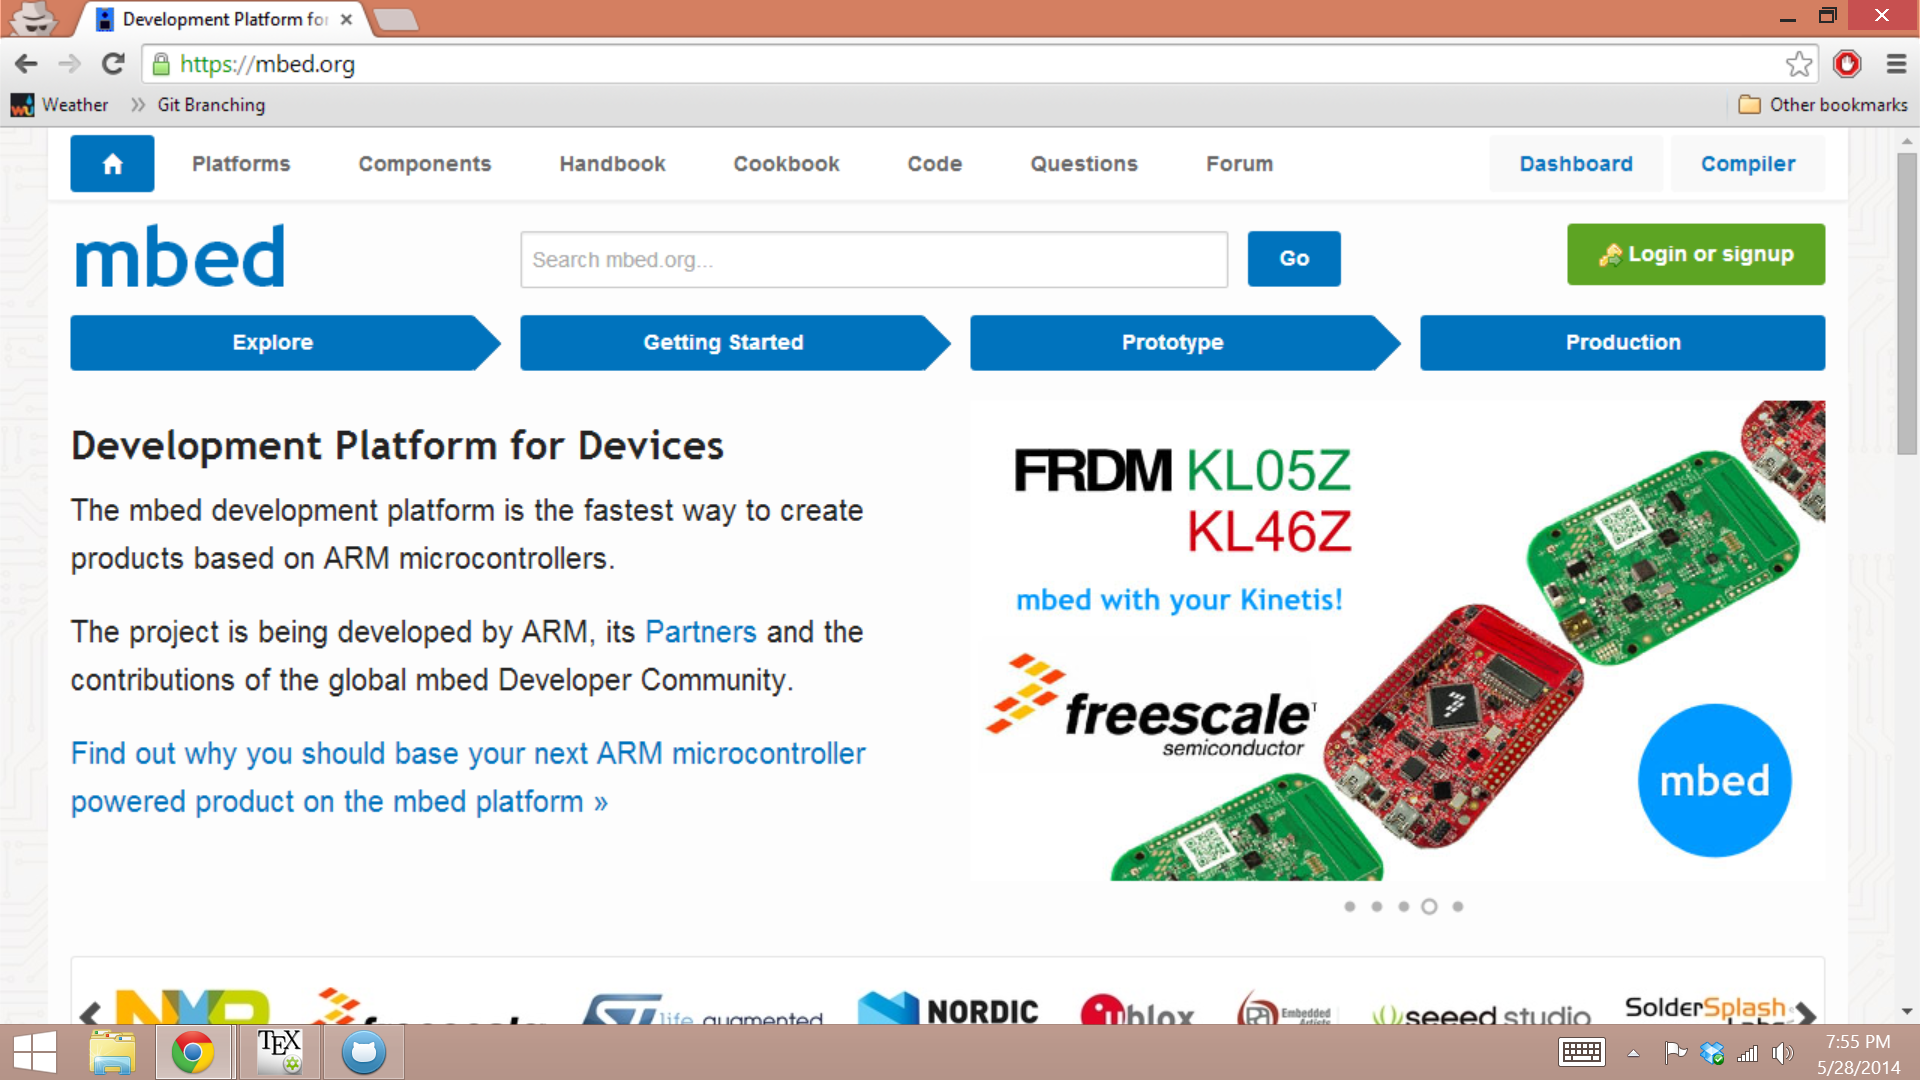
\includegraphics[width=\linewidth]{part_1/mbed_register}
		\end{column}
		\begin{column}{0.5\textwidth}
			\begin{enumerate}
				\item Navigate to \url{http://www.mbed.org}
				\item Click the green login or signup button
				\item Click the signup button
				\item Follow the prompts
				\item Confirm your e-mail address
			\end{enumerate}
		\end{column}
	\end{columns}
	\vspace{1ex}
	Everyone should have an account on mbed.
	You can create a team to share programs between users in your organization.
\end{frame}

\subsection{Nucleo Development Board}
\begin{frame}
	\frametitle{Nucleo Development Board}
	\begin{columns}[T]
		\begin{column}{0.5\textwidth}
			The Nucleo development board combines a USB programmer with a powerful STM32 processor and Arduino compatible headers
			\begin{itemize}
				\item ARM Cortex-M4 with FPU at 84 MHz
				\item 512 KBytes flash memory
				\item 12bit ADC at 2.4 Msps with up to 10 channels
				\item Up to 3xUART, 3xI2C, 4xSPI interfaces
			\end{itemize}
		\end{column}
		\begin{column}{0.5\textwidth}
			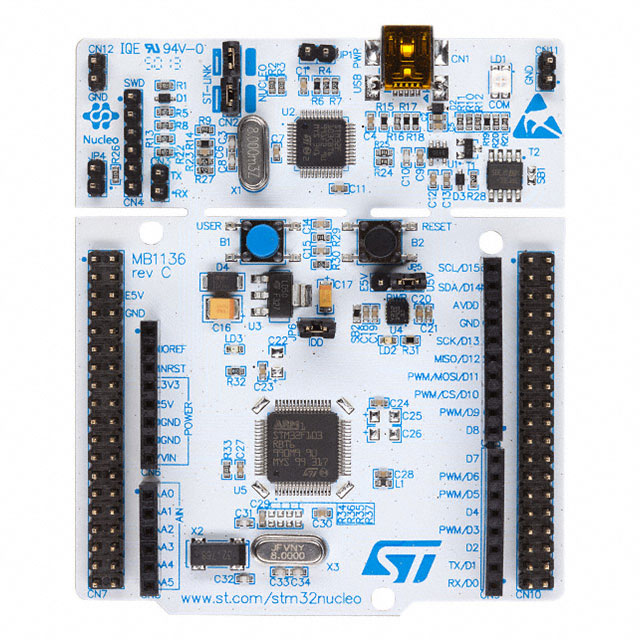
\includegraphics[width=\linewidth]{part_1/nucleo}
		\end{column}
	\end{columns}
\end{frame}

\begin{frame}
	\frametitle{Add Nucleo to Your Account}
	\begin{columns}[c]
		\begin{column}{0.5\textwidth}
			%TODO Edit add_nucleo
			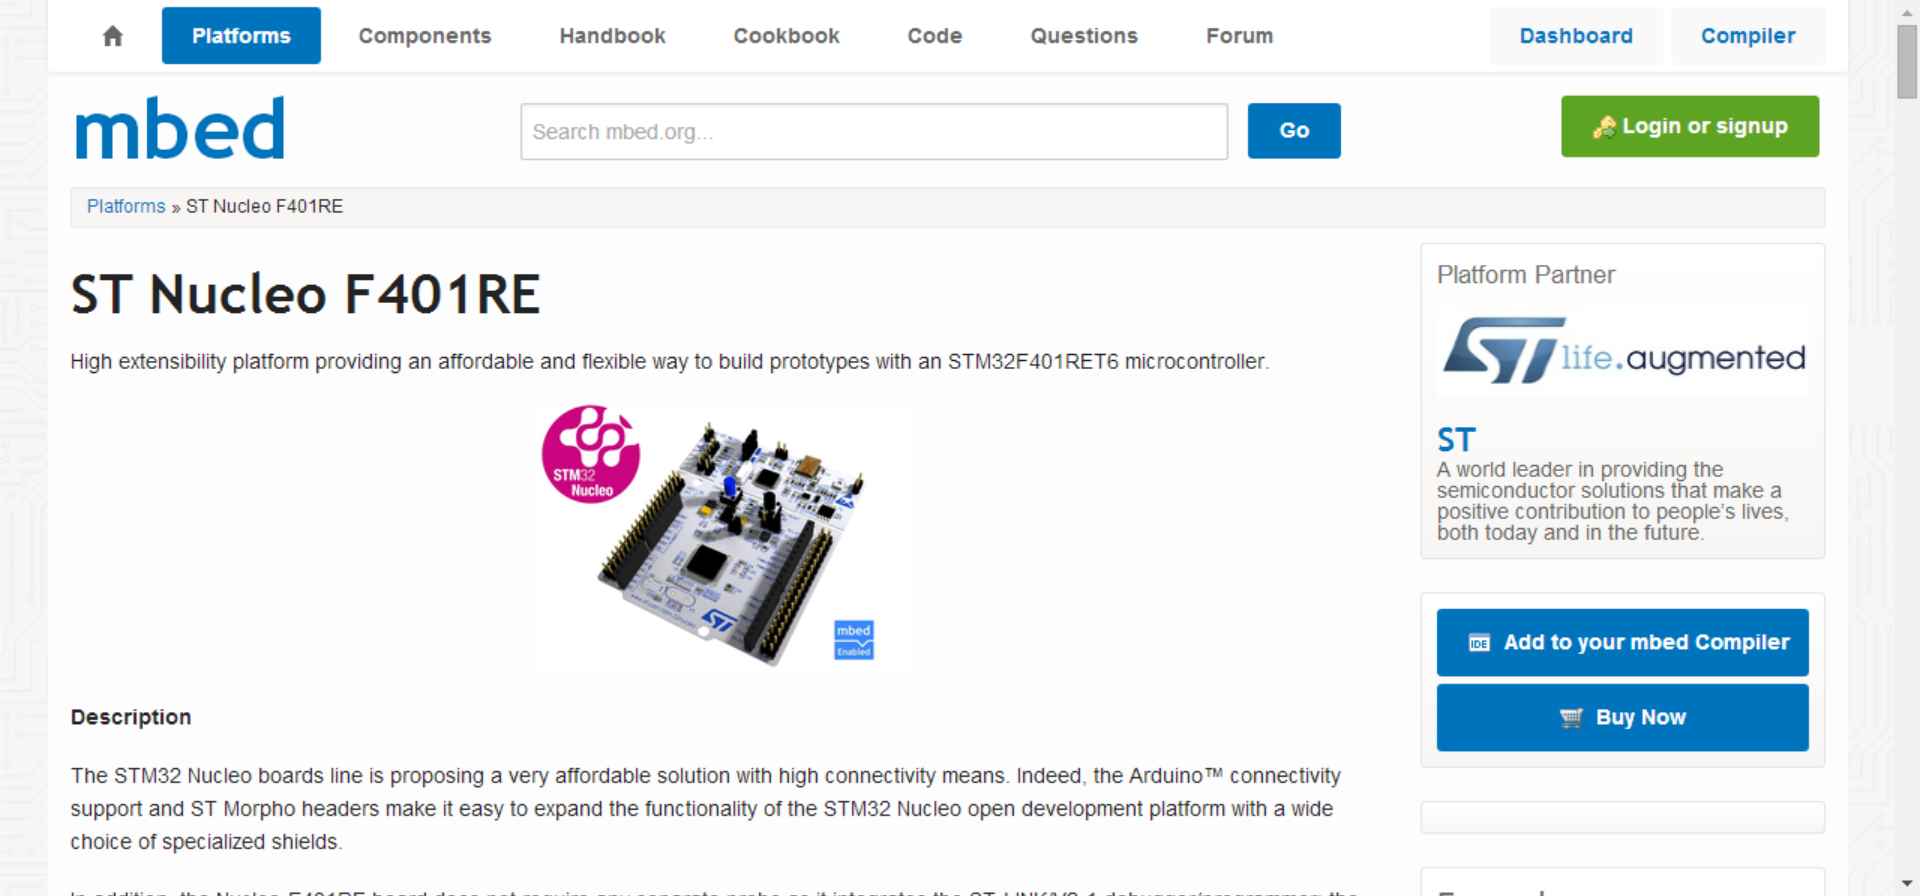
\includegraphics[width=\linewidth]{part_1/add_nucleo}
		\end{column}
		\begin{column}{0.5\textwidth}
			\begin{enumerate}
				\item Connect your Nucleo to your computer
				\item Open the external drive that connects
				\item Open the mbed.htm file
				\item Click "Add to Your mbed Compiler"
				%TODO add nucleo to compiler steps
			\end{enumerate}
		\end{column}
	\end{columns}
	\begin{block}{Notice}
		You only need to do this once!
	\end{block}
\end{frame}

\subsection{An Example Program}
\begin{frame}
	\frametitle{An Example Program}
	\begin{columns}[T]
		\begin{column}{0.5\textwidth}
			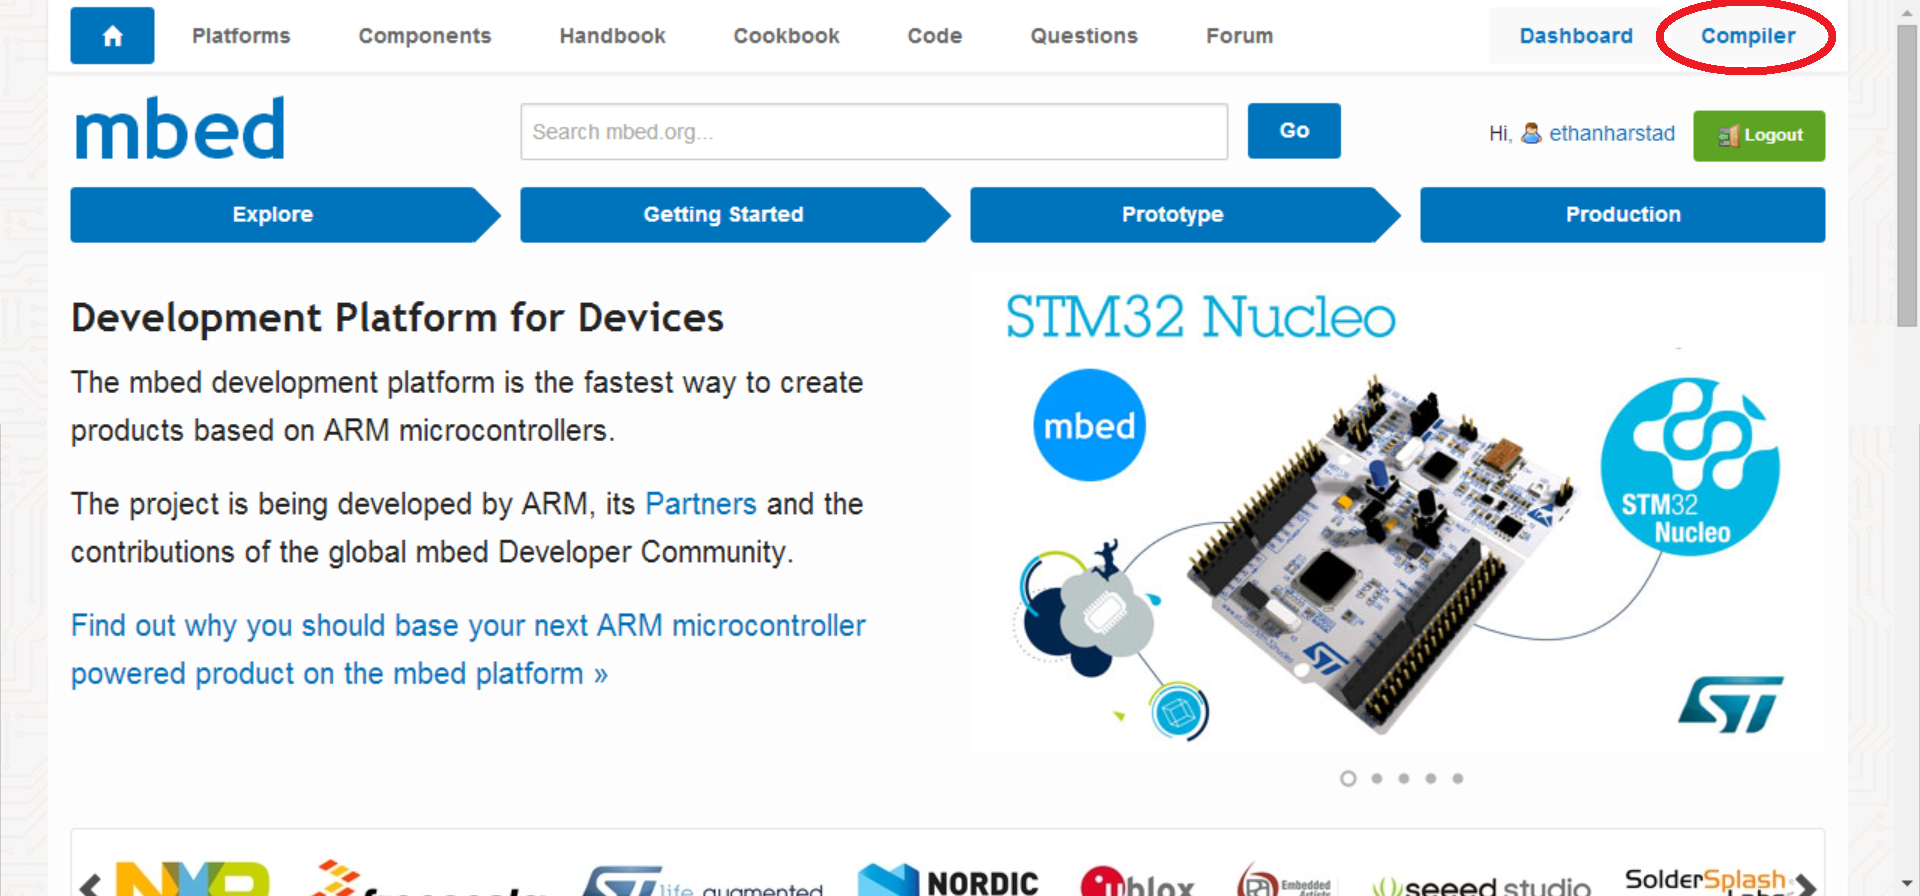
\includegraphics[width=\linewidth]{part_1/open_compiler}
			\vspace{1ex}
			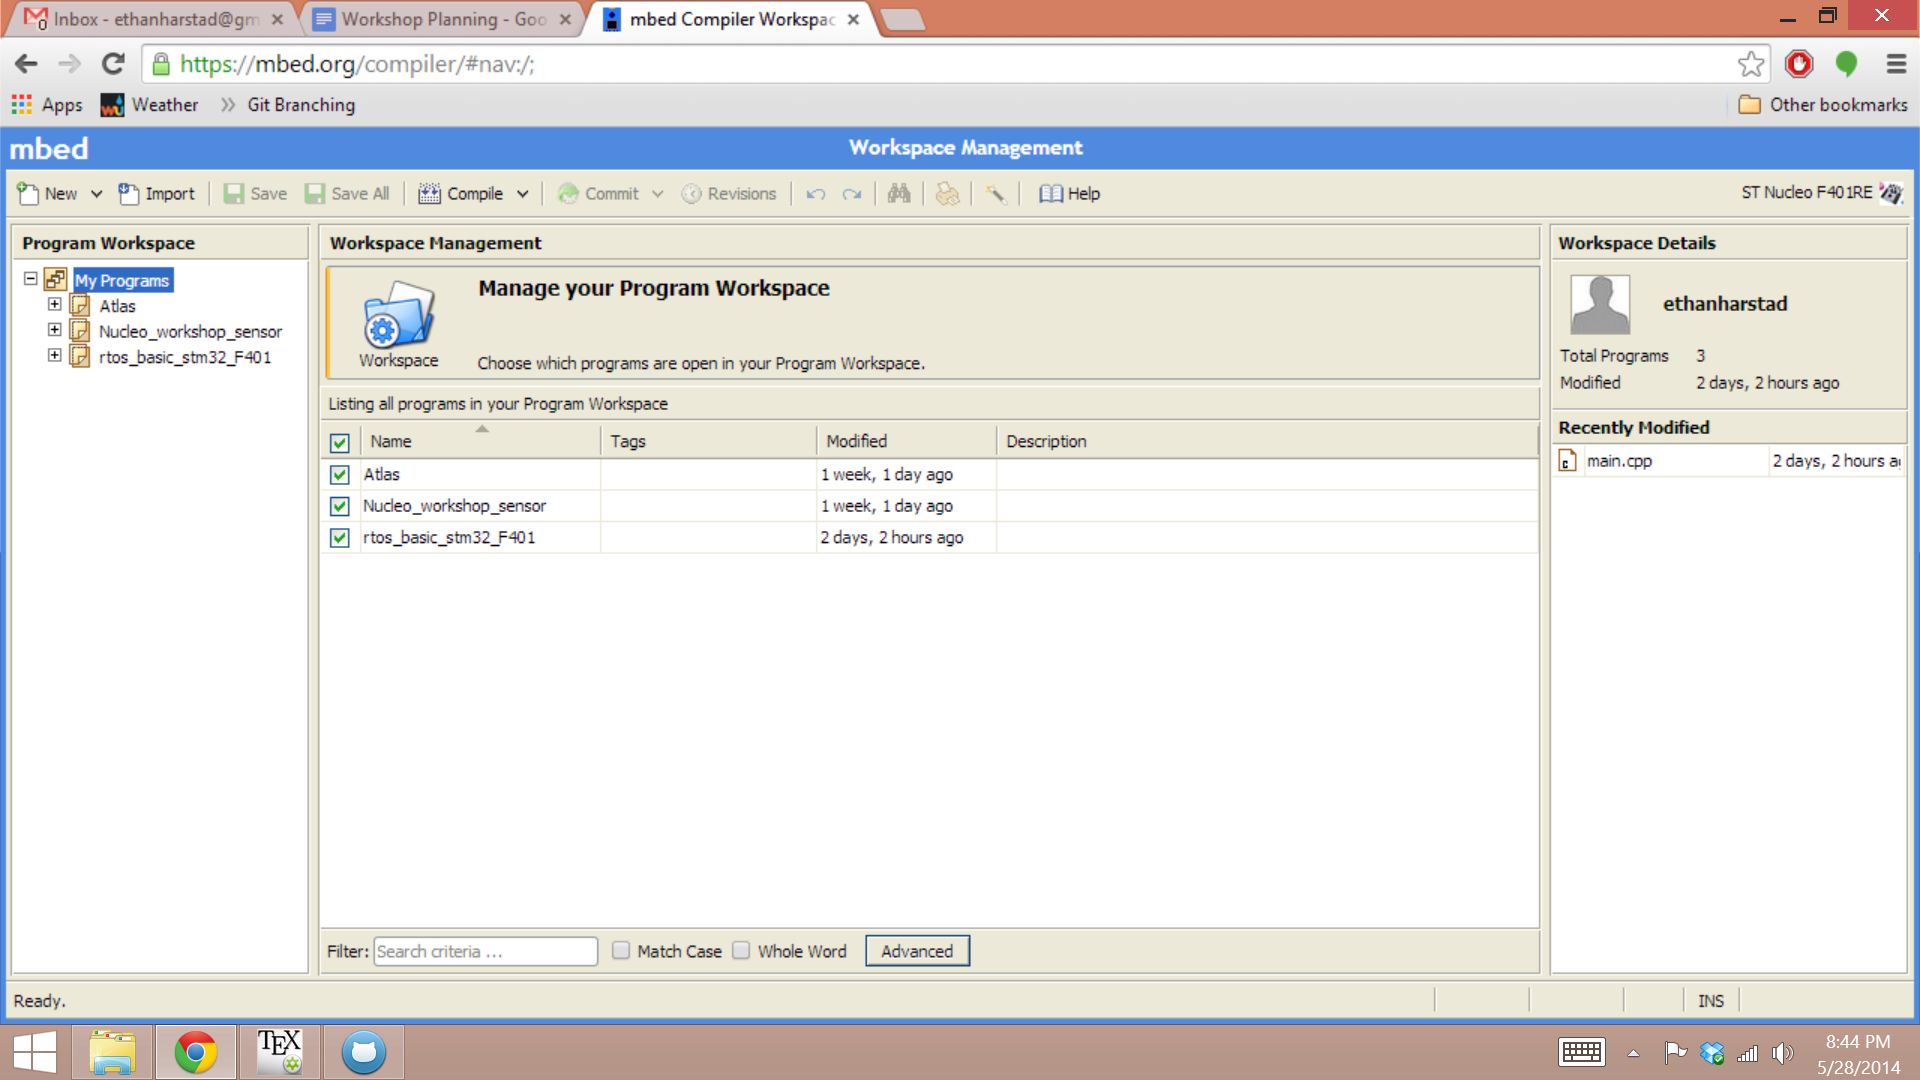
\includegraphics[width=\linewidth]{part_1/new_project}
		\end{column}
		\begin{column}{0.5\textwidth}
			\begin{enumerate}
				\item Navigate to \url{http://www.mbed.org}
				\item Click the Compiler button
				\item Click New and select New Program
				\item Choose "Blinky LED" as the program template
				\item Name the program anything you desire and click OK
			\end{enumerate}
		\end{column}
	\end{columns}
\end{frame}

\begin{frame}
	\frametitle{Compile and Upload Your Program}
	\begin{columns}[T]
		\begin{column}{0.5\textwidth}
			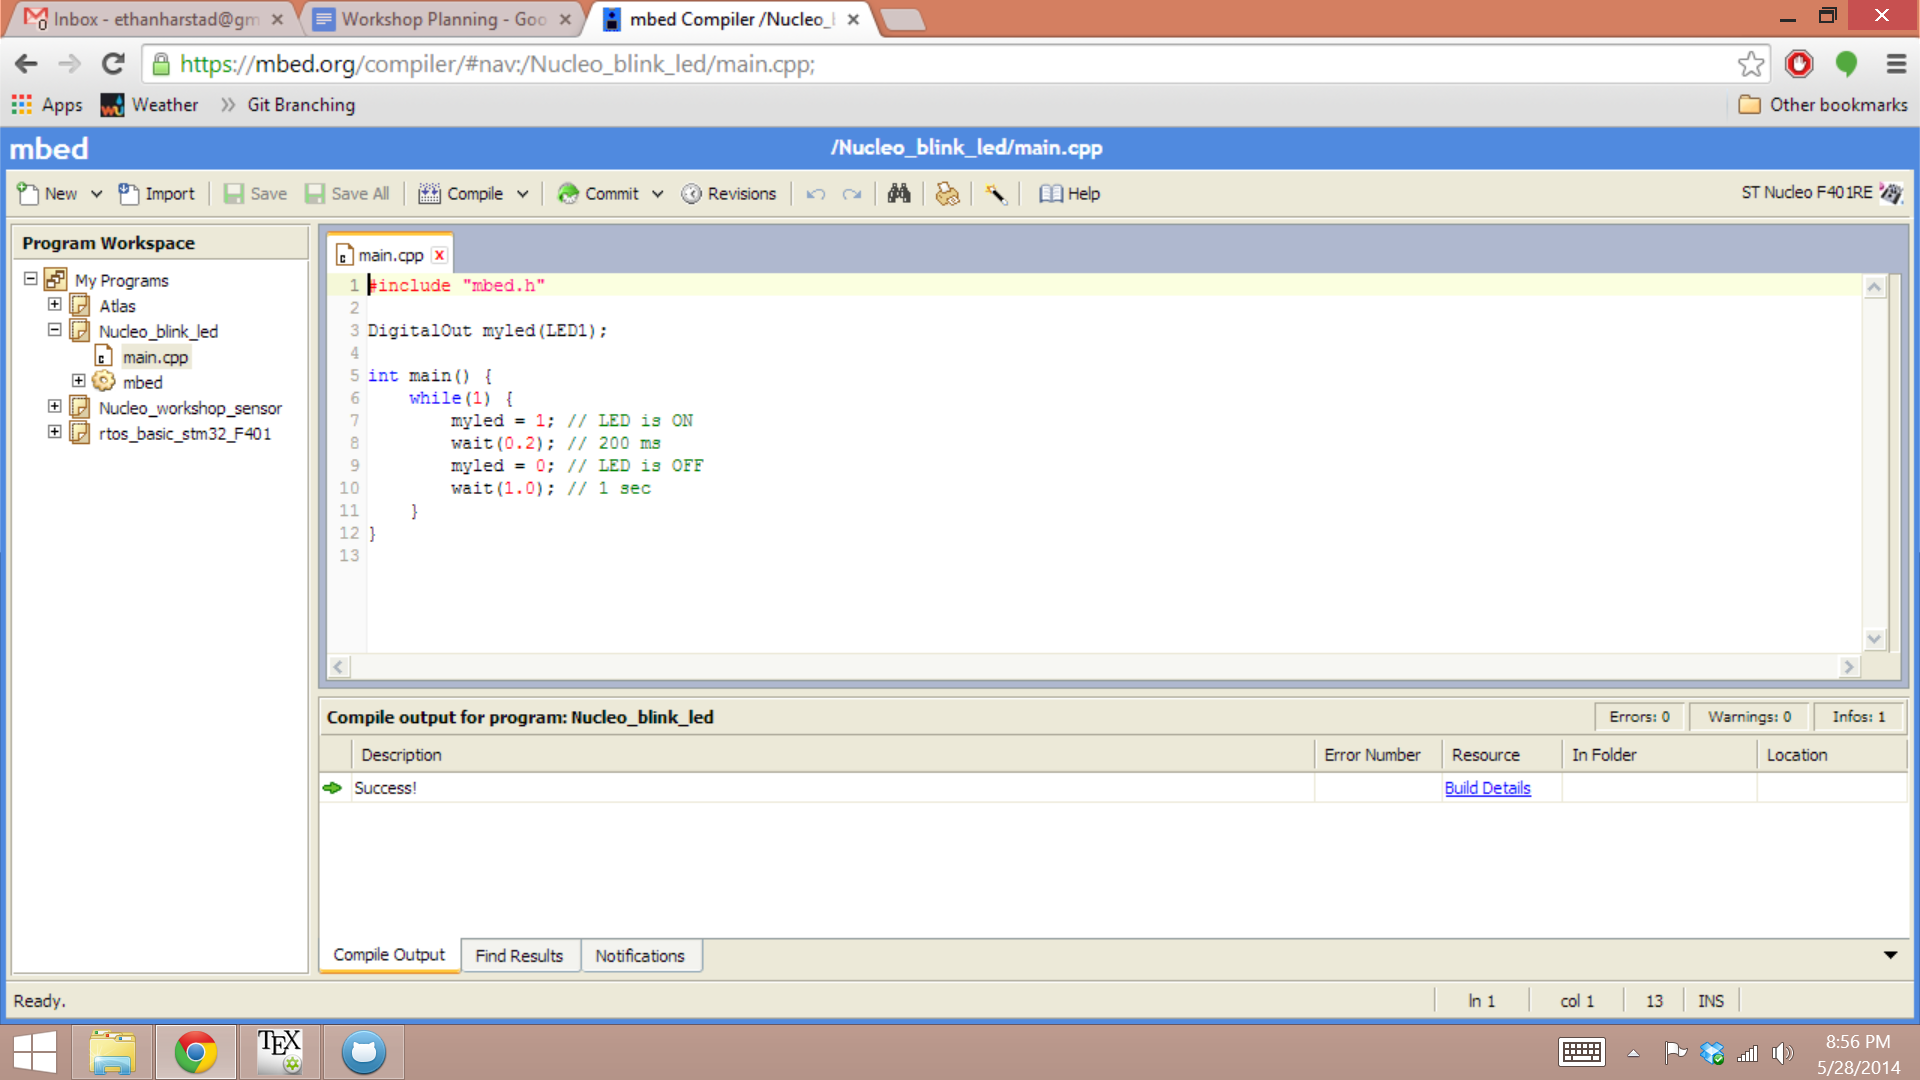
\includegraphics[width=\linewidth]{part_1/compile_program}
			\begin{block}{Tip}
				Set your browsers download location to the Nucleo to save time while debugging
			\end{block}
		\end{column}
		\begin{column}{0.5\textwidth}
			\begin{enumerate}
				\item Click Compile
				\item A file will be downloaded
				\item Move this file to the Nucleo external drive
				\item The LED will flash red/green while programming
				\item When the` LED is solid green, your program has started successfully!
			\end{enumerate}
		\end{column}
	\end{columns}
\end{frame}

\section{mbed Basics}
\subsection{Your Own Program}
\begin{frame}
	\frametitle{Create an Empty Program}
	\begin{columns}[T]
		\begin{column}{0.5\textwidth}
			%TODO Edit import_library
			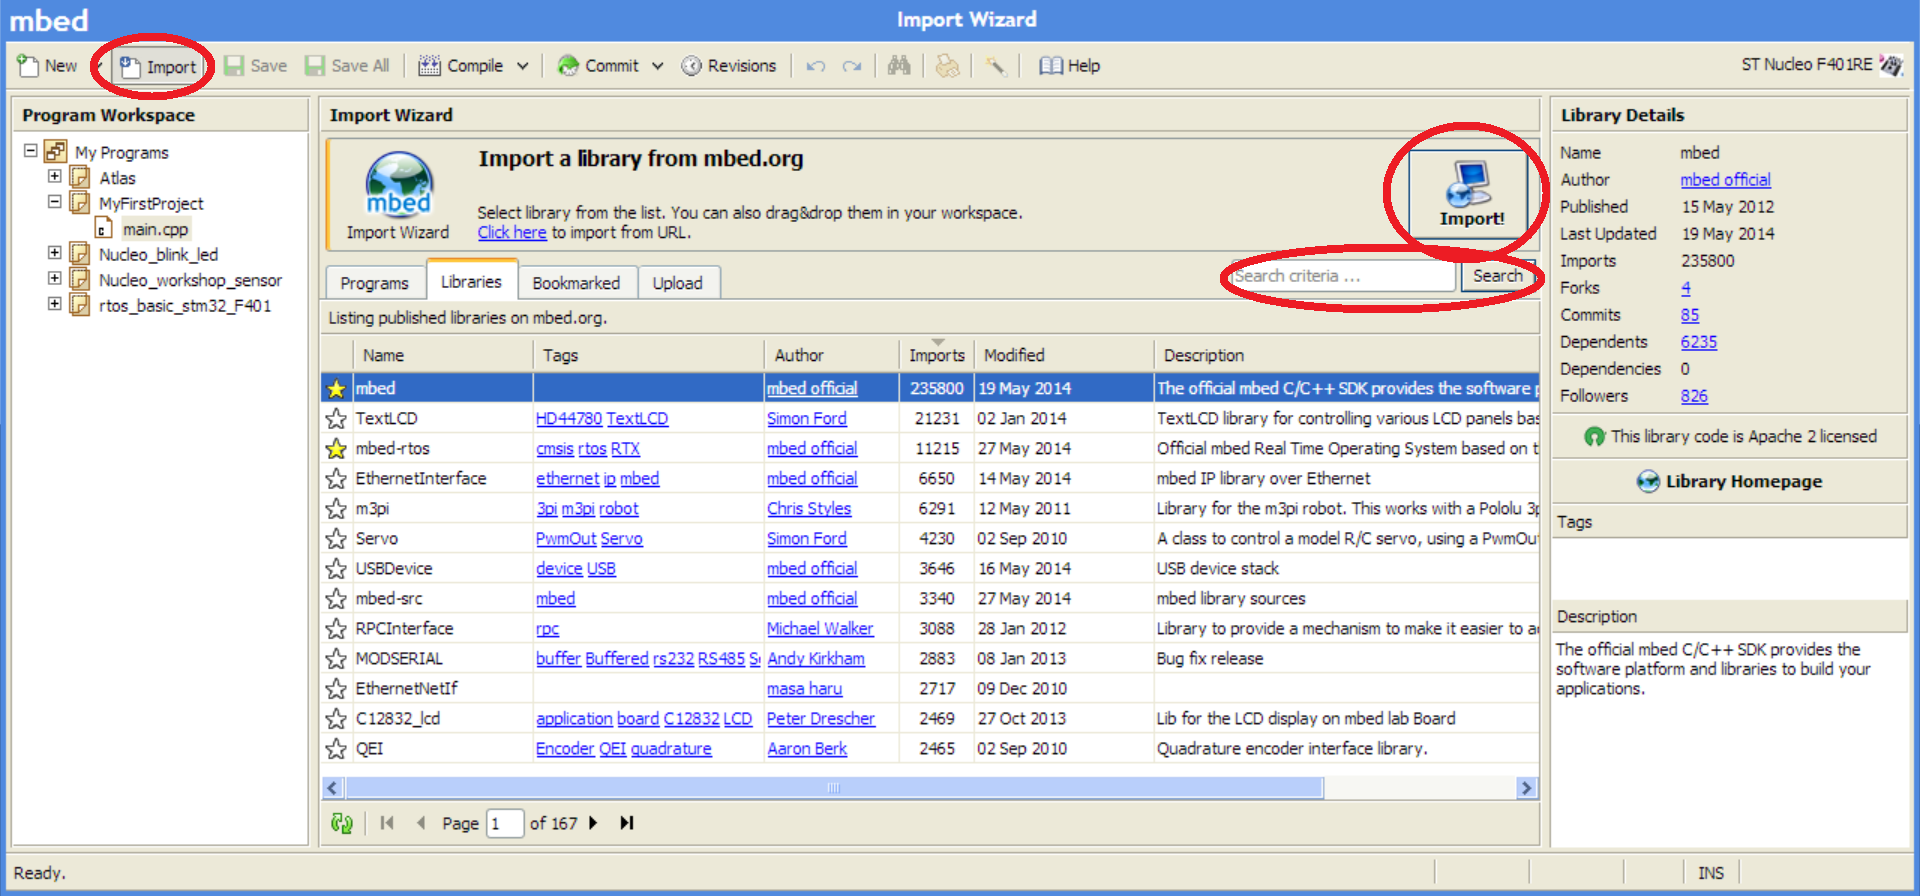
\includegraphics[width=\linewidth]{part_1/import_library}
		\end{column}
		\begin{column}{0.5\textwidth}
			\begin{enumerate}
				\item Create a new program with "Empty Program" as the template
				\item Create a new file named "main.cpp"
				\item Click Import and search for "mbed"
			\end{enumerate}
		\end{column}
	\end{columns}
	\begin{block}{Notice}
		The mbed library is required for every mbed based program
	\end{block}
\end{frame}

\begin{frame}[fragile]
	\frametitle{Write Your First Program}
	\lstinputlisting[caption=main.cpp]{snippets/first_program/1.cpp}
\end{frame}

\begin{frame}[fragile]
	\frametitle{Breaking Down main.cpp}
	\lstinputlisting[firstline=1, lastline=1, firstnumber=1]{snippets/first_program/1.cpp}
	\lstinline{#include} directive is used to include another file, in this case "mbed.h".
	You will use this to include libraries in your program.
	You can also split your program into multiple files and combine them using the include directive.
	
	\lstinputlisting[firstline=3, lastline=3, firstnumber=3]{snippets/first_program/1.cpp}
	\lstinline{DigitalOut} is a class from the mbed library that supports digital output.
	The library also provides \lstinline{DigitalIn} and \lstinline{DigitalInOut} for inputs and bidirection pins.
	This line creates an object named \lstinline{led} that is attached to the \lstinline{LED1} pin.
\end{frame}

\begin{frame}[fragile]
	\frametitle{Breaking Down main.cpp}
	\lstinputlisting[firstline=5, lastline=5, firstnumber=5]{snippets/first_program/1.cpp}
	This line declares a function called \lstinline{main} that takes no parameters and returns an integer.
	Every program needs a function with this signature, it is used as the entry point to the program.
	
	\lstinputlisting[firstline=6, lastline=6, firstnumber=6]{snippets/first_program/1.cpp}
	This is an example of a type of loop.
	It runs while the condition inside the parentheses is true, in the case, always.
	This loop will never terminate because a microcontroller program should never exit.
\end{frame}

\begin{frame}[fragile]
	\frametitle{Breaking Down main.cpp}
	\lstinputlisting[firstline=7, lastline=10, firstnumber=7]{snippets/first_program/1.cpp}
	This is what makes the LED flash.\\
	Writing a 1 to an output pin sets the pin high, and a 0 sets the pin low.
	\lstinline{wait(sec)} is a function provided by the mbed library that halts the program.
	\begin{block}{Try It Yourself}
		Try changing the wait times or making your own patterns.
	\end{block}
\end{frame}